%\documentclass[9pt]{elife}
\documentclass[multi=figure,9pt]{standalone}
\usepackage{graphicx}

\RequirePackage[T1]{fontenc}
\RequirePackage[utf8]{inputenc}
\RequirePackage{stix}
\RequirePackage[default]{opensans}
\renewcommand{\ttdefault}{lmtt}

\RequirePackage{microtype}

% Trueno/Open Sans requires a bigger "single" linespread.
\linespread{1.2}
\if@onehalfspacing\linespread{1.5}\fi
\if@doublespacing\linespread{2.0}\fi

\RequirePackage{graphicx,xcolor}
\definecolor{eLifeDarkBlue}{HTML}{273B81}
\definecolor{eLifeLightBlue}{HTML}{0A9DD9}
\definecolor{eLifeMediumGrey}{HTML}{6D6E70}
\definecolor{eLifeLightGrey}{HTML}{929497}

\RequirePackage{booktabs}
\RequirePackage{authblk}

\RequirePackage{changepage}

\RequirePackage{silence}
\WarningFilter{caption}{The option `hypcap=true' will be ignored}

\RequirePackage[labelfont={bf},%
                labelsep=period,%
                justification=raggedright,%
                singlelinecheck=true,%
                tableposition=top,font={color=eLifeDarkBlue,scriptsize}]
                {caption}

\makeatletter
\renewenvironment{figure}%
{\def\@captype{figure}%
\minipage{\textwidth}}%
{\endminipage}
\makeatother

\let\efloatseparator=\empty

\usepackage{subcaption}

\begin{document}

\begin{figure}
    \centering
    \captionsetup[subfigure]{font={color=eLifeDarkBlue,footnotesize}}
    \begin{subfigure}[b]{0.49\textwidth}
            \centering
           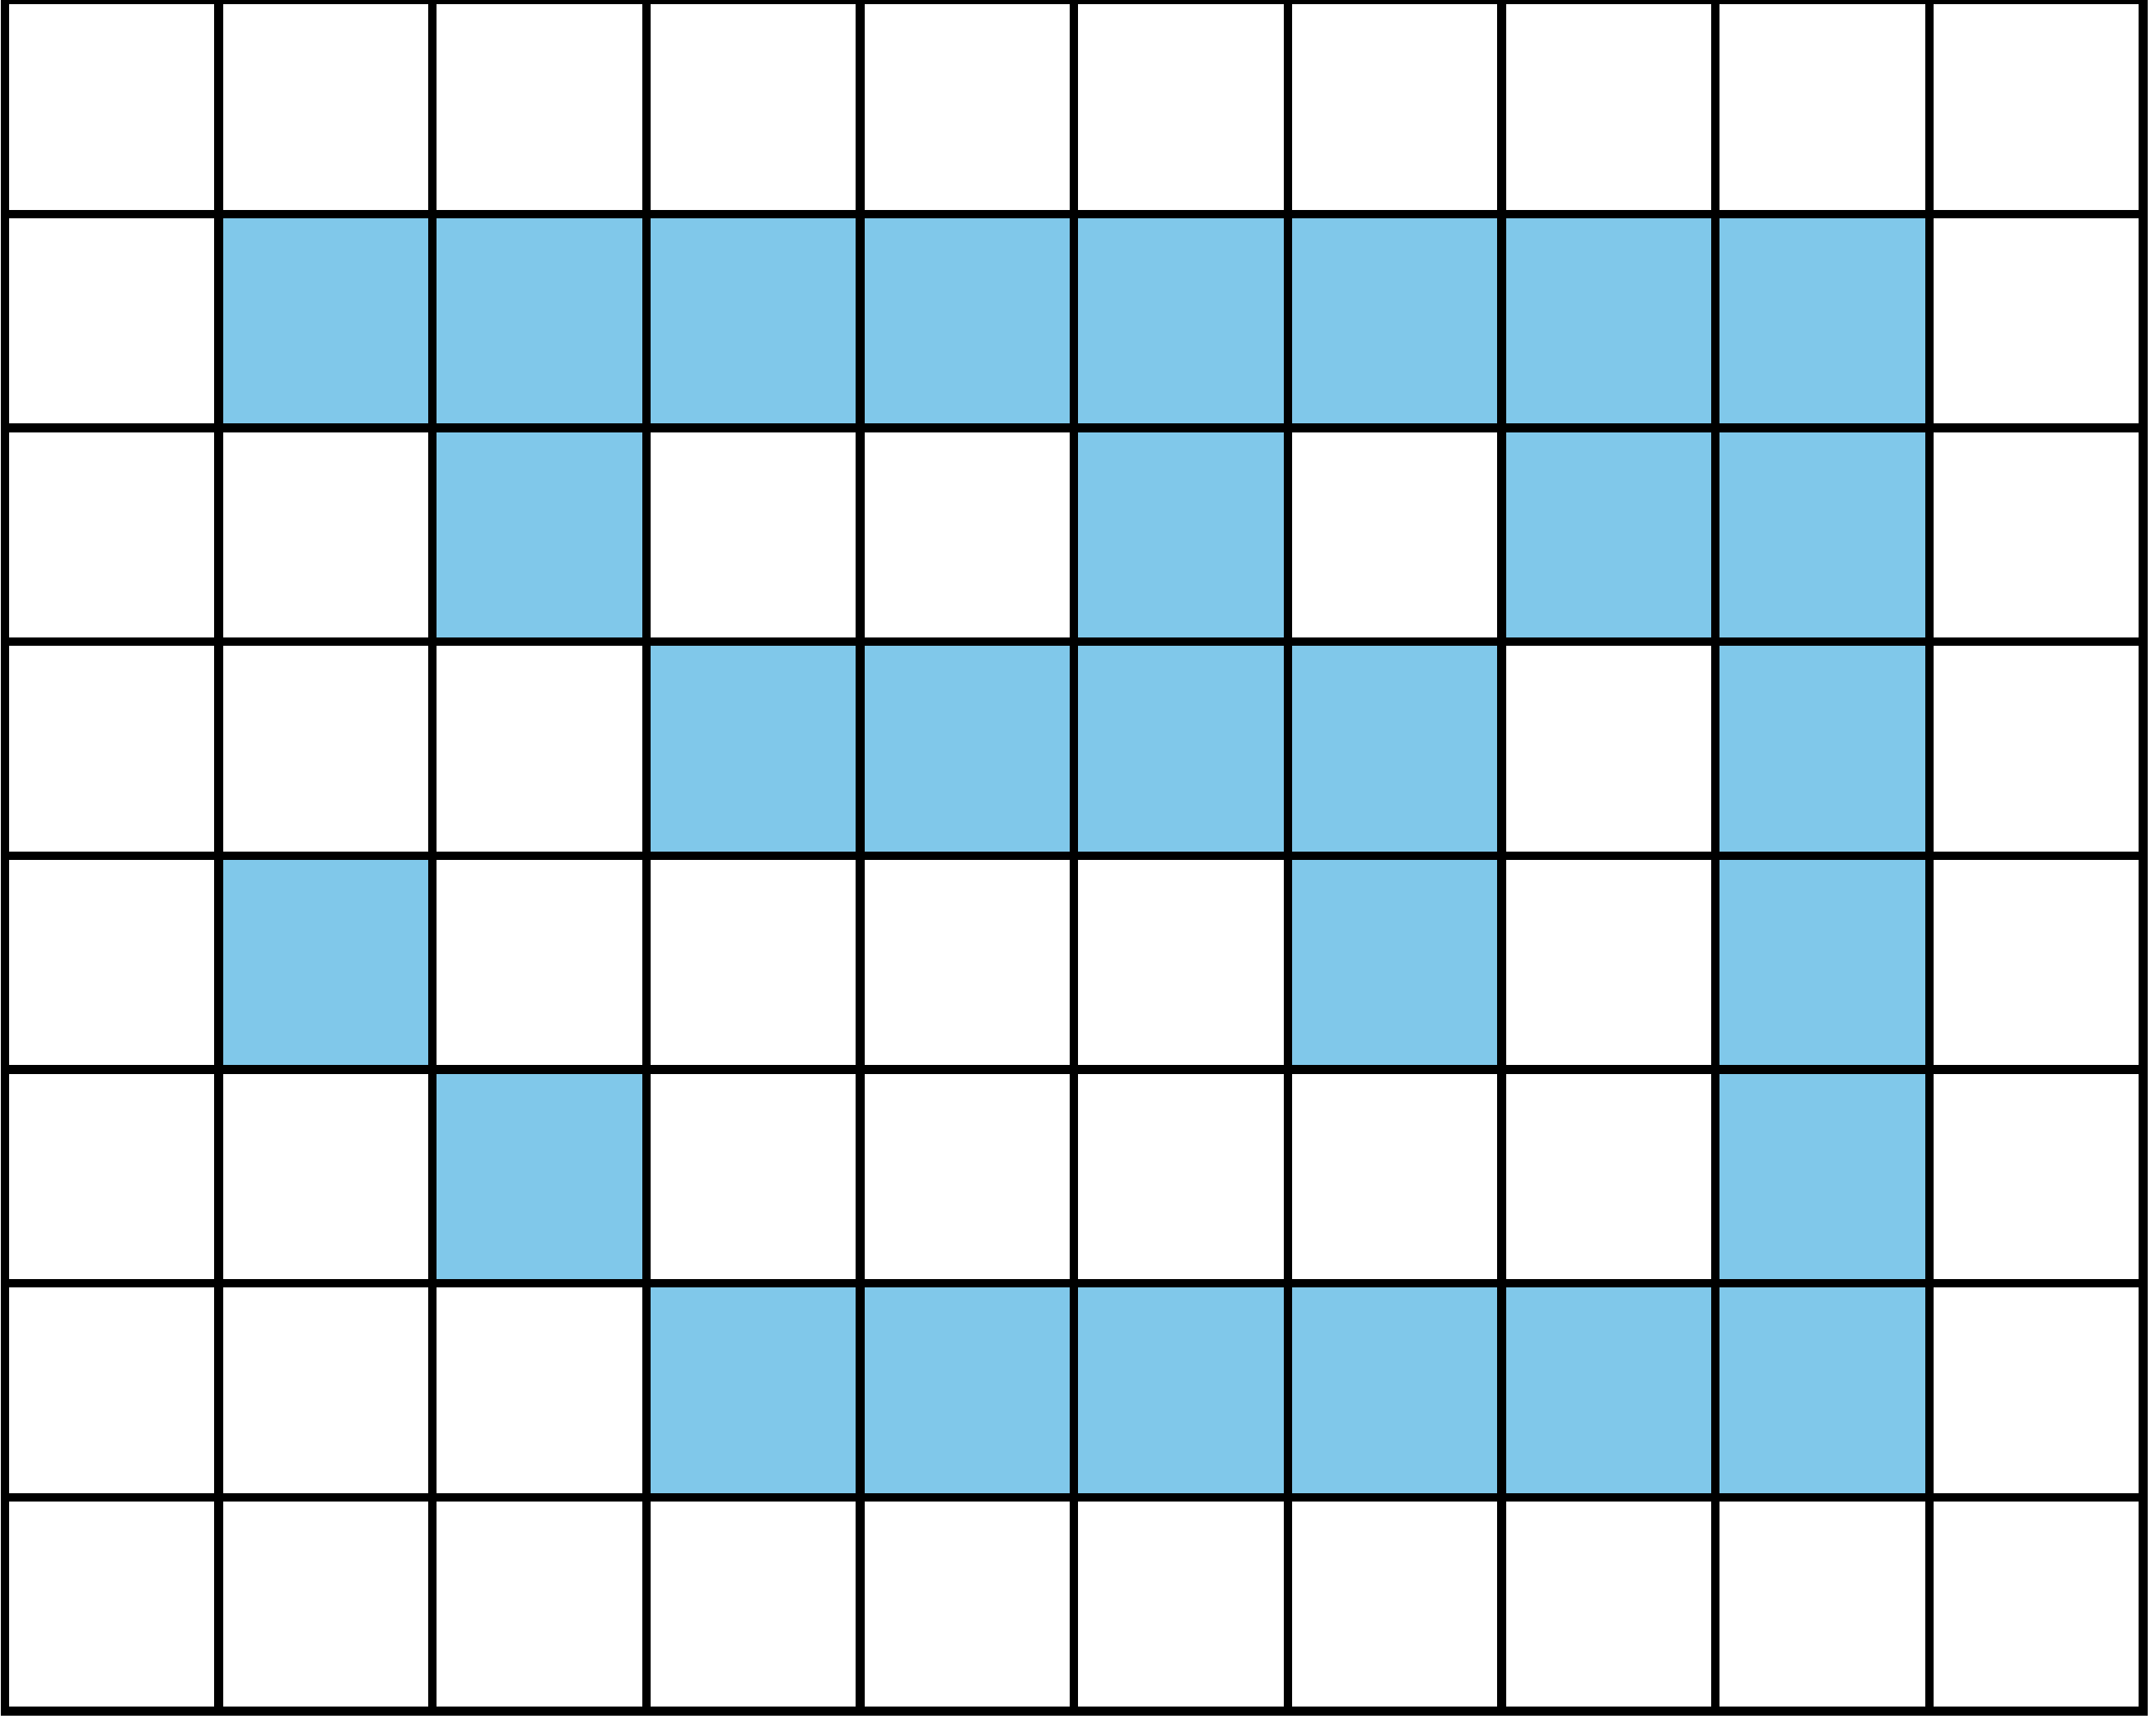
\includegraphics[width=\textwidth]{piece.pdf}
           % \caption{Original image with colors in Viridis color-scheme.}
            %\label{fig:outlinea}
    \end{subfigure}
    \begin{subfigure}[b]{0.49\textwidth}
           \centering
            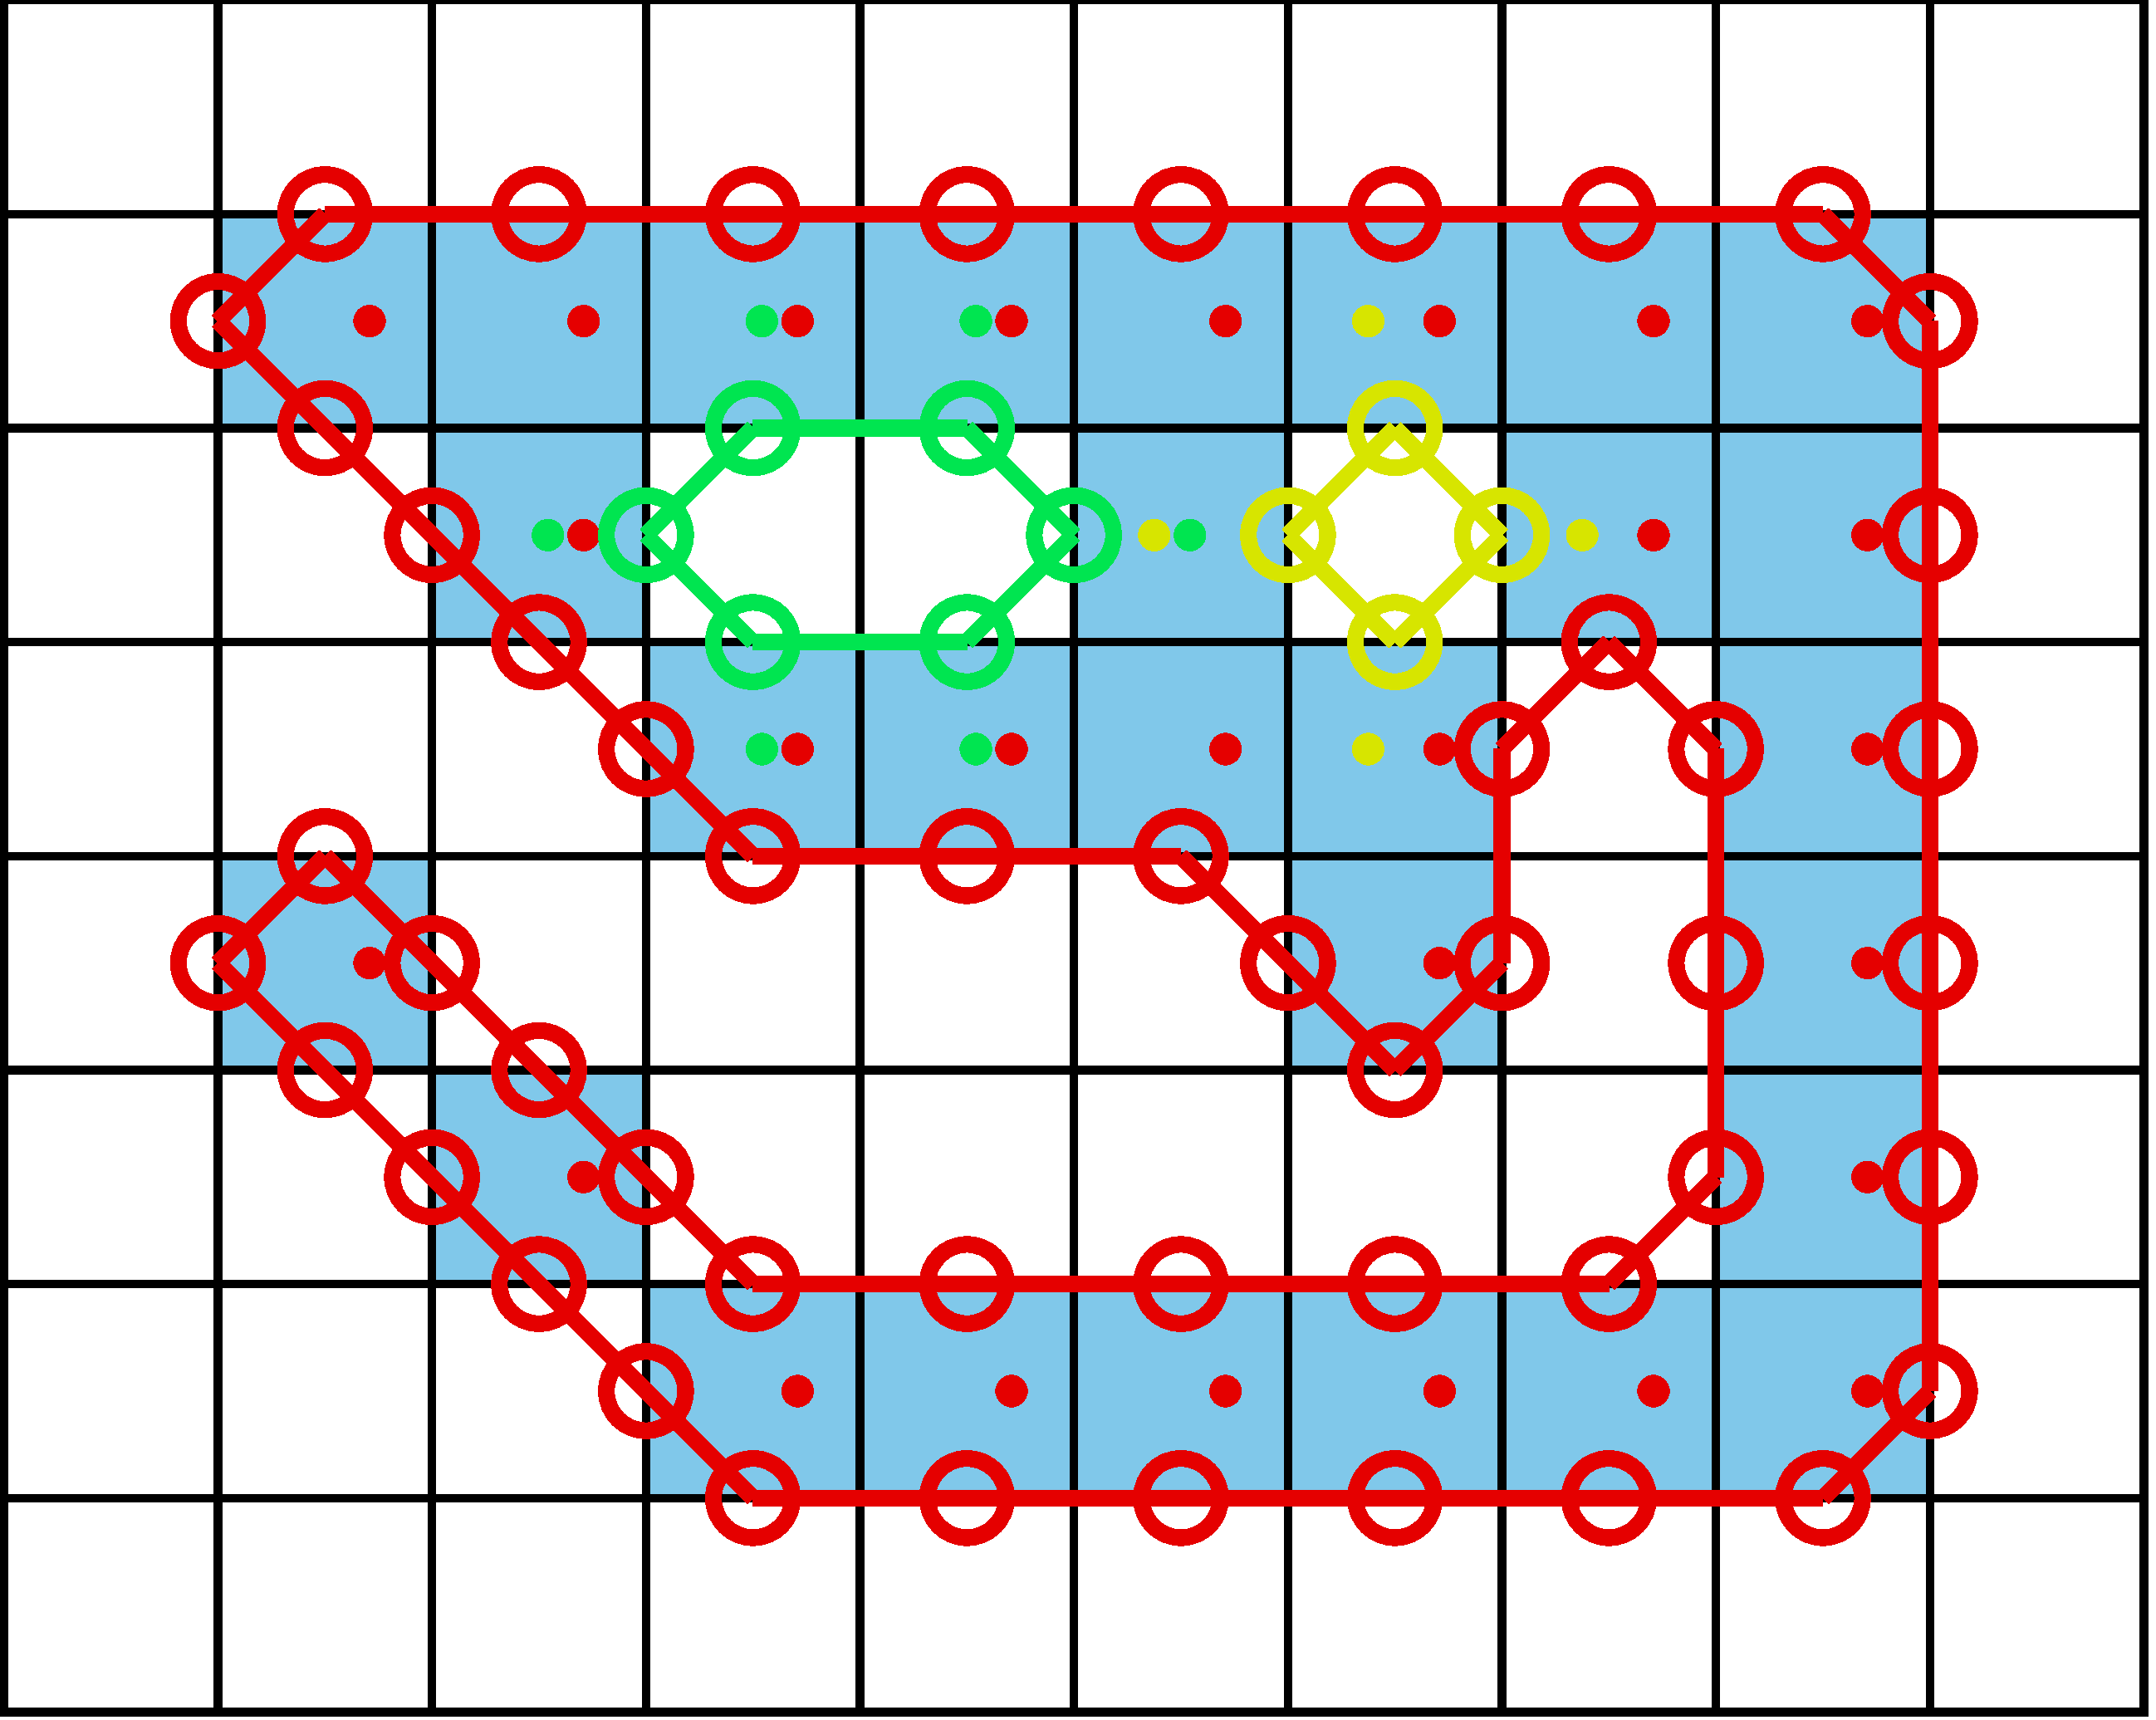
\includegraphics[width=\textwidth]{outline_approximation.pdf}
            %\caption{Outlines found by \TRex{}' algorithm.}
           % \label{fig:outlineb}
    \end{subfigure}
\end{figure}

\end{document}